\documentclass[paper=a4,fontsize=12pt,parskip=half*]{scrartcl}

\usepackage[utf8]{inputenc}				
\usepackage[T1]{fontenc}
\usepackage{graphicx}
\usepackage{babel}
\usepackage{amsmath}
\usepackage[a4paper,left=25mm,right=35mm,top=25mm,bottom=30mm]{geometry}
\usepackage{hyperref}
\usepackage{enumitem}
\usepackage{amssymb} 
\usepackage{subcaption}
\usepackage{cite}

\usepackage{xcolor} % For colors
\usepackage{float} % For float positioning
\usepackage{pgfplots} % For charts and plots
\pgfplotsset{compat=1.18}

\begin{document}

% Define a small filled rectangle symbol
\newcommand{\rectangle}{\rule{0.5em}{0.5em}}

\pagenumbering{roman}
\pagestyle{plain}

% Einbinden der Titelseite
\begin{titlepage}

    \linespread{1.5}

    
\includegraphics[width=\linewidth]{graphics/htw_logo}

    \begin{center}
        \large
        \hfill
        \vfill
        \Large{\bfseries{The Game Library Manager}}

        von \\ Yahya E. Selo Matrikel Nr. 5013655 \\ Sherwan Diko Matrikel Nr. 5013656
        \\ Clarita Kawam Matrikel Nr. 5013484  \\ Bayan Alshami Matrikel Nr. 5011108 

        \vfill

        Ein Projekt Bericht im Rahmen der Vorlesung\\ \glqq Programmierung 3
        (PIB-PR3)\grqq\\ an der htw saar im Studiengang Informatik\\

        \vfill
        \vfill

        Saarbrücken, \today
    \end{center}

\end{titlepage}


% Hier ist der Abstract
\section*{Summary}

The Game Library Manager is a software application designed for managing personal or shared
game collections. It provides features such as adding, editing, and deleting games, tracking progress
and statistics, and offering a user-friendly, text-based interface. The application employs a
robust three-layer architecture to facilitate maintenance and extensibility. Persistent data storage is
implemented using an SQLite database, abstracted with the help of jOOQ\footnote{Why You Should Use jOOQ With Code Generation\cite{JOOQ}}.
This document outlines the requirements, design, and implementation strategy of the application.
% Das Inhaltsverzeichnis
\clearpage
\tableofcontents

\clearpage
\pagenumbering{arabic}

% Hier beginnt das erste Kapitel

\section{Project Overview}
\begin{itemize}
	\item \textbf{Project Name:} Game Library Manager
	\item \textbf{Objective:} To provide users with an organized system to track and manage their game collections, progress, and multiplayer statistics.
	\item \textbf{Target Audience:} Gamers and collectors.
\end{itemize}

\section{Requirements}

\subsection{Must-Have Requirements}
\begin{enumerate}
	\item \textbf{Core Functionalities:}
	      \begin{itemize}
		      \item Add, edit, and delete games from the library.
		      \item Search and filter games by title, genre, or platform.
		      \item Track gameplay progress and multiplayer statistics.
		      \item Allow users to rate and review games.
		      \item Provide recommendations based on user preferences and borrowing history.
	      \end{itemize}
	\item \textbf{Persistence:}
	      \begin{itemize}
		      \item Store data in a local SQLite database.
		      \item Use jOOQ to abstract database interactions.
	      \end{itemize}
	\item \textbf{User Interface:}
	      \begin{itemize}
		      \item Text-based user interface (CLI or TUI).
		      \item Platform-independent implementation.
	      \end{itemize}
	\item \textbf{Three-Layer Architecture:}
	      \begin{itemize}
		      \item \textbf{Presentation Layer:} Handles user interaction.
		      \item \textbf{Logic Layer:} Contains business logic for managing the library.
		      \item \textbf{Persistence Layer:} Manages data storage and retrieval.
	      \end{itemize}
\end{enumerate}

\subsection{Should-Have Requirements}
\begin{enumerate}
	\item Integration of gamification elements like achievements.
	\item Detailed analytics and statistics about game usage.
	\item Export/import functionalities for game data.
	\item Integration with external APIs (e.g., Steam or Xbox Live) to automatically pull game data.
	\item Advanced search functionalities (e.g., search by release date, developer, or rating).
\end{enumerate}

\subsection{Can-Have Requirements}
\begin{enumerate}
	\item Optional graphical user interface (GUI).
	\item Integration with a game engine (e.g., Unity or Unreal) for virtual game previews.
	\item Multiplayer statistics tracking (e.g., win/loss ratios, leaderboards).
	\item Cloud-based synchronization for game libraries across multiple devices.
\end{enumerate}

\section{Design and Architecture}

\subsection{Three-Layer Architecture}
\begin{itemize}
	\item \textbf{Presentation Layer:} Handles user interaction through a text-based interface (CLI or TUI).
	\item \textbf{Logic Layer:} Contains the business logic for managing the game library, including adding, editing, and deleting games, as well as tracking progress and statistics.
	\item \textbf{Persistence Layer:} Manages data storage and retrieval using a SQLite database and jOOQ for database abstraction.
\end{itemize}

\subsection{Model-View-Controller (MVC) Pattern}
\begin{itemize}
	\item \textbf{Model:} Manages the data and business logic of the application (e.g., game details, user ratings).
	\item \textbf{View:} Displays the data to the user (e.g., game list, search results).
	\item \textbf{Controller:} Mediates between the Model and View, processing user input and updating the Model and View accordingly.
\end{itemize}

\begin{figure}[!ht]
	\centering
	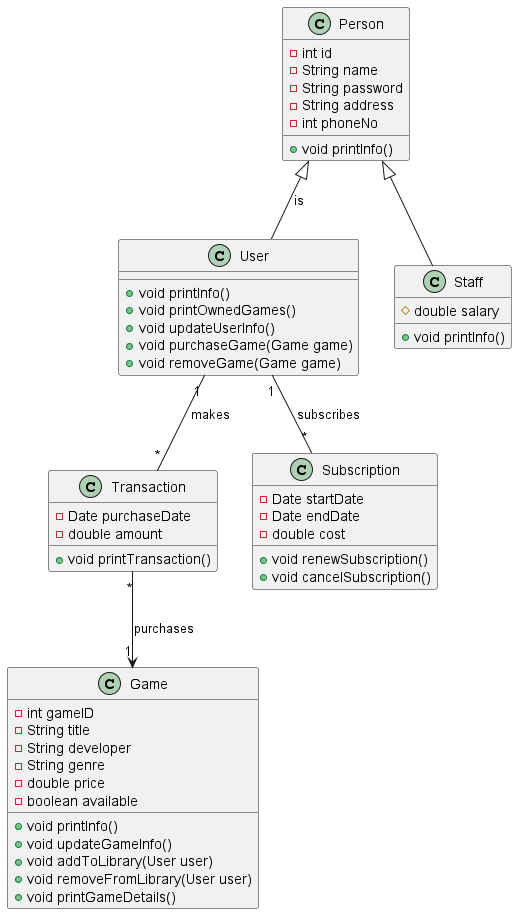
\includegraphics[width=0.8\textwidth]{out/graphics/Charts/Klassendiagramm/Klassendiagramm.png}
	\caption{(Class Diagram)}
	\label{fig:class}
\end{figure}

\subsection{Database Design}
\begin{itemize}
	\item \textbf{Entities:}
	      \begin{itemize}
		      \item \textbf{Game:} Title, Genre, Platform, Availability, Rating, Review.
		      \item \textbf{User:} Gamer profile, Borrowing history, Preferences.
		      \item \textbf{Loan:} Game borrowed, User, Due date, Return status.
	      \end{itemize}
	\item \textbf{Relationships:}
	      \begin{itemize}
		      \item A User can borrow multiple Games.
		      \item A Game can be borrowed by multiple Users.
	      \end{itemize}
\end{itemize}


\pagebreak

%################################################################################
%TODO: Change the following text to the actual Installation details
%################################################################################

\section{Quick Start Guide}
\subsection*{Installation}
\begin{enumerate}
	\item Clone the repository.
	\item Install dependencies using Maven\cite{Maven}.
	\item Install Java 17 or higher.\cite{Java}
	\item Build the project.
\end{enumerate}

\subsection{Running the Application}
\begin{enumerate}
	\item Run the application using the command: \texttt{java -jar GameLibraryManager.jar}
	\item Follow the on-screen instructions to navigate the menu.
\end{enumerate}

% Hier beginnt das Literaturverzeichnis
\clearpage
\renewcommand\refname{Literaturverzeichnis}
\bibliographystyle{alpha}
\bibliography{literatur}
\addcontentsline{toc}{section}{Literaturverzeichnis}

\end{document}